\subsection{Množinové operace}
\label{ssec:mnozinove-operace}

Podobně jako na výrocích, i na množinách lze provádět různé operace. V rámci
jejich vnímání jako \emph{souborů} je přirozené, že takové soubory umíme
slučovat, oddělovat a vybírat z více souborů pouze prvky jim všem společné. Tyto
tři základní množinové operace se zde jmeme připomenout.

Jsou-li $A,B$ množiny, pak
\begin{itemize}
 \item \emph{sjednocením} $A$ a $B$, zapsaným $A \cup B$, myslíme množinu, která
  obsahuje prvky ležící aspoň v~jedné z těchto množin; logicky, $A \cup B$ je
  množina splňující výrok
  \[
   (x \in A \cup B) \Leftrightarrow (x \in A \vee x \in B).
  \]
 \begin{figure}[ht]
  \centering
  \begin{subfigure}{.45\textwidth}
   \centering
   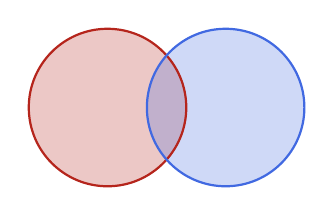
\begin{tikzpicture}[scale=0.5]
    \fill[BrickRed,fill opacity=0.25] (180:1.5) circle (2);
    \fill[RoyalBlue,fill opacity=0.25] (0:1.5) circle (2);
    \draw[BrickRed,thick] (180:1.5) circle (2);
    \draw[RoyalBlue,thick] (0:1.5) circle (2);
   \end{tikzpicture}
   \caption{Množiny $\clr{A}$ a $\clb{B}$.}
   \label{subfig:sjednoceni-a}
  \end{subfigure}
  \begin{subfigure}{.45\textwidth}
   \centering
   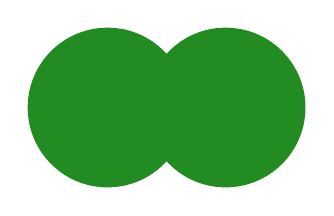
\begin{tikzpicture}[scale=0.5]
    \def\firstcircle{(180:1.5) circle (2)}
    \def\secondcircle{(0:1.5) circle (2)}
    \filldraw[thick,ForestGreen] \firstcircle; 
    \filldraw[thick,ForestGreen] \secondcircle;
   \end{tikzpicture}
   \caption{Sjednocení $\clg{A \cup B}$.}
   \label{subfig:sjednoceni-b}
  \end{subfigure}
  \caption{Operace sjednocení množin.}
  \label{fig:sjednoceni}
 \end{figure}
 \item \emph{průnikem} $A$ a $B$, zapsaným $A \cap B$, myslíme množinu
  obsahující pouze prvky ležící v obou množinách; logicky, $A \cap B$ je množina
  splňující
  \[
   (x \in A \cap B) \Leftrightarrow (x \in A \wedge x \in B).
  \]
  \begin{figure}[ht]
   \centering
   \begin{subfigure}{.45\textwidth}
    \centering
    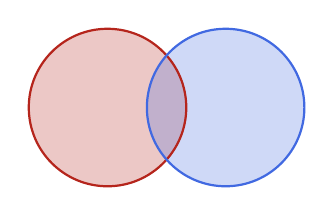
\begin{tikzpicture}[scale=0.5]
     \fill[BrickRed,fill opacity=0.25] (180:1.5) circle (2);
     \fill[RoyalBlue,fill opacity=0.25] (0:1.5) circle (2);
     \draw[BrickRed,thick] (180:1.5) circle (2);
     \draw[RoyalBlue,thick] (0:1.5) circle (2);
    \end{tikzpicture}
    \caption{Množiny $\clr{A}$ a $\clb{B}$.}
    \label{subfig:prunik-a}
   \end{subfigure}
   \begin{subfigure}{.45\textwidth}
    \centering
    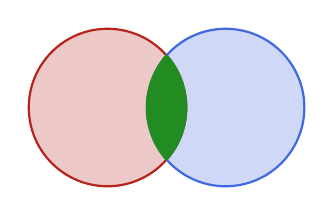
\begin{tikzpicture}[scale=0.5]
     \def\firstcircle{(180:1.5) circle (2)}
     \def\secondcircle{(0:1.5) circle (2)}
     
     \fill[BrickRed,fill opacity=0.25] \firstcircle;
     \fill[RoyalBlue,fill opacity=0.25] \secondcircle;
     \draw[BrickRed,thick] \firstcircle;
     \draw[RoyalBlue,thick] \secondcircle;

     \begin{scope}
      \clip \firstcircle;
      \fill[white] \secondcircle;
      \filldraw[thick,ForestGreen] \secondcircle;
     \end{scope}
     \begin{scope}
      \clip \secondcircle;
      \draw[ForestGreen,thick] \firstcircle;
     \end{scope}
    \end{tikzpicture}
    \caption{Průnik $\clg{A \cap B}$.}
    \label{subfig:prunik-b}
   \end{subfigure}
   \caption{Operace průniku množin.}
   \label{fig:prunik}
  \end{figure}
 \item \emph{rozdílem} $A$ a $B$, zapsaným $A \setminus B$, myslíme množinu
  obsahující prvky ležící v $A$, které však neleží v $B$; logicky, $A \setminus
  B$ je množina splňující
  \[
   (x \in A \setminus B) \Leftrightarrow (x \in A \wedge x \notin B).
  \]
  \begin{figure}[ht]
   \centering
   \begin{subfigure}{.3\textwidth}
    \centering
    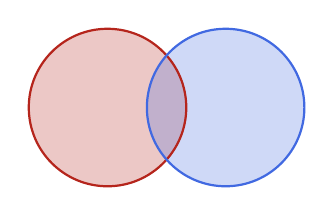
\begin{tikzpicture}[scale=0.5]
     \fill[BrickRed,fill opacity=0.25] (180:1.5) circle (2);
     \fill[RoyalBlue,fill opacity=0.25] (0:1.5) circle (2);
     \draw[BrickRed,thick] (180:1.5) circle (2);
     \draw[RoyalBlue,thick] (0:1.5) circle (2);
    \end{tikzpicture}
    \caption{Množiny $\clr{A}$ a $\clb{B}$.}
    \label{subfig:rozdil-a}
   \end{subfigure}
   \begin{subfigure}{.3\textwidth}
    \centering
    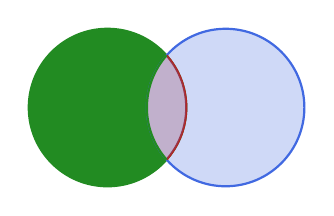
\begin{tikzpicture}[scale=0.5]
     \def\firstcircle{(180:1.5) circle (2)}
     \def\secondcircle{(0:1.5) circle (2)}
     
     \filldraw[thick,ForestGreen] \firstcircle;
     \fill[RoyalBlue,fill opacity=0.25] \secondcircle;
     \draw[RoyalBlue,thick] \secondcircle;

     \begin{scope}
      \clip \secondcircle;
      \fill[white] \firstcircle;
      \fill[BrickRed,fill opacity=0.25] \firstcircle;
      \draw[BrickRed,thick] \firstcircle;
     \end{scope}
     \begin{scope}
      \clip \firstcircle;
      \fill[RoyalBlue,fill opacity=0.25] \secondcircle;
      \draw[ForestGreen,thick] \secondcircle;
     \end{scope}
    \end{tikzpicture}
    \caption{Rozdíl $\clg{A \setminus B}$.}
    \label{subfig:rozdil-b}
   \end{subfigure}
   \begin{subfigure}{.3\textwidth}
    \centering
    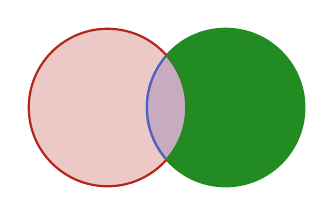
\begin{tikzpicture}[scale=0.5]
     \def\firstcircle{(0:1.5) circle (2)}
     \def\secondcircle{(180:1.5) circle (2)}
     
     \filldraw[thick,ForestGreen] \firstcircle;
     \fill[BrickRed,fill opacity=0.25] \secondcircle;
     \draw[BrickRed,thick] \secondcircle;

     \begin{scope}
      \clip \secondcircle;
      \fill[white] \firstcircle;
      \fill[RoyalBlue,fill opacity=0.25] \firstcircle;
      \draw[RoyalBlue,thick] \firstcircle;
     \end{scope}
     \begin{scope}
      \clip \firstcircle;
      \fill[BrickRed,fill opacity=0.25] \secondcircle;
      \draw[ForestGreen,thick] \secondcircle;
     \end{scope}
    \end{tikzpicture}
    \caption{Rozdíl $\clg{B \setminus A}$.}
    \label{subfig:rozdil-c}
   \end{subfigure}
   \caption{Operace rozdílu množin.}
   \label{fig:rozdil}
  \end{figure}
  Je dobré dbát faktu, že $A \setminus B$ a $B \setminus A$ jsou obecně
  \textbf{různé} množiny.
\end{itemize}

Operace sjednocení a průniku mají své \uv{hromadné} varianty, tedy sjednocení a
průnik většího (klidně nekonečného) počtu množin. V případech jako je tento, kdy
potřebujeme provádět operace na libovolném množství objektů, se často užívá
pomocné množiny, tzv. \emph{množiny indexů}, která slouží jen k tomu, aby
jednotlivé objekty v operované skupině od sebe odlišovala.

Konkrétně, zápisem
\[
 \bigcup_{i \in I} A_i,\text{ resp.}\bigcap_{i \in I} A_i,
\]
myslíme množinu, která obsahuje prvky, které leží aspoň v jedné, resp. v každé,
z množin $A_i,i \in I$, kde $I$ je libovolná množina indexů. K formální logické
definici je třeba použít kvantifikátorů, neboť množina $I$ nemusí mít konečně
prvků. Definujeme
\[
 (x \in \bigcup_{i \in I} A_i) \Leftrightarrow (\exists i \in I:x \in A_i)
\]
a
\[
 (x \in \bigcap_{i \in I} A_i) \Leftrightarrow ( \forall i \in I:x \in A_i).
\]
Tyto definice jsou původem matematické pranostiky \uv{Existenční kvantifikátor
je sjednocení a universální kvantifikátor je průnik.}

Ve speciálním případě, kdy $I = \{1,\ldots,n\}$ je množina přirozených čísel od
$1$ do $n$, se také užívá zápisů
\[
 \bigcup_{i = 1}^{n} A_i \quad \text{a} \quad \bigcap_{i = 1}^{n} A_i.
\]

Není obtížné si uvědomit, že pro rozdíl taková definice není možná, neboť u
rozdílu množin záleží na jejich pořadí a, opakujeme (vizte
\myref{výstrahu}{warn:mnozina-bez-poradi}), množina indexů $I$ \emph{neurčuje
pořadí}, v~kterém se množiny $A_i$ sjednocují či pronikají.

Dalším oblíbeným způsobem zápisu těchto operací, především v teorii kategorií,
je $\bigcup \mathcal{A}$ a $\bigcap \mathcal{A}$, kde $\mathcal{A} \coloneqq
\{A_i \mid i \in I\}$ je pomocná množina všech množin $A_i,i \in I$.
\textbf{Pozor!} Množina $\mathcal{A}$ není v~žádném smyslu sjednocením množin
$A_i$; je to množina, která má za prvky ony samotné množiny $A_i$, ne jejich
prvky. Obecně, žádný prvek žádné množiny $A_i$ není zároveň prvkem
$\mathcal{A}$, speciálně $A_i$ obecně \textbf{nejsou} podmnožiny $\mathcal{A}$.
